\def\linkdethi{} %Đường link cần dẫn tới
\anmaQR
%%%%%%%%%%%%%%%%%%%%%%%%
\def\toanlop{12}
\def\thoigian{90}
\def\namhoc{2025 - 2026}
\begin{dethi}
	{Bộ GD\&ĐT}
	{VTED ft KING EDU}
	{TDMZZ03}
	{Đề thi thử THPTQG 2026}
\end{dethi}
\caulc
\Opensolutionfile{ans}[ans/ansTN-Dung]
%%%=============EX_1=============%%%
\begin{ex}%[1D6N4-2]%[TDMZZ03]%[Mui Doan]
	Tập nghiệm của phương trình $2^{x^4-1}=32\,768$ là
	\choice
	{\True $\pm 2$}
	{$\pm 3$}
	{$\pm 4$}
	{$\pm 5$}
	\loigiai{
		Ta có $2^{x^4-1}=32\,768\Leftrightarrow 2^{x^4-1}=2^{15}\Leftrightarrow x^4-1=15\Leftrightarrow x^4=16\Leftrightarrow x=\pm 2$.
	}
\end{ex}
%%%=============================%%%

%%%=============EX_2=============%%%
\begin{ex}%[1D2H3-4]%[TDMZZ03]%[Huỳnh Trí Thiện]
	Cho cấp số nhân $\left(u_n\right)$ có số hạng đầu bằng $2$ và số hạng thứ ba bằng $8$. Khẳng định luôn đúng là
	\choice
	{$u_2 = 4$}
	{$u_4 = -16$}
	{\True $u_5 = 32$}
	{$q = 2$}
	\loigiai{
		Ta có $u_3 = u_1 \cdot q^2 \Leftrightarrow 8 = 2 \cdot q^2 \Leftrightarrow q^2 = 4$.\\
		Suy ra $u_5 = u_1 \cdot q^4 = 2 \cdot \left(q^2\right)^2 = 2 \cdot 4^2 = 32$.
	}
\end{ex}
%%%=============================%%%

%%%=============EX_3=============%%%
\begin{ex}%[1D3H2-5]%[TDMZZ03]%[Chu Hà]
	Giới hạn $\lim\limits_{x\to -\infty}\left(\sqrt{x^2-2x}+x\right)$ bằng
	\choice
	{\True $1$}
	{$-1$}
	{$0$}
	{$+\infty$}
	\loigiai{
		Ta có\allowdisplaybreaks
		\begin{eqnarray*}
			&&\lim\limits_{x\to -\infty}\left(\sqrt{x^2-2x}+x\right)
			=\lim\limits_{x\to -\infty}\dfrac{\left(\sqrt{x^2-2x}+x\right)\left(\sqrt{x^2-2x}-x\right)}{\sqrt{x^2-2x}-x}\\
			&=&\lim\limits_{x\to -\infty}\dfrac{x^2-2x-x^2}{\sqrt{x^2-2x}-x}
			=\lim\limits_{x\to -\infty}\dfrac{-2x}{\sqrt{x^2-2x}-x}.
		\end{eqnarray*}
		Ta có $\sqrt{x^2-2x}=|x|\sqrt{1-\dfrac{2}{x}}$.\\
		Vì $x\to -\infty$ nên $|x|=-x$, suy ra
		$\sqrt{x^2-2x}=-x\sqrt{1-\dfrac{2}{x}}$.\\
		Khi đó\allowdisplaybreaks
		\begin{eqnarray*}
			\dfrac{-2x}{\sqrt{x^2-2x}-x}
			=\dfrac{-2x}{-x\sqrt{1-\dfrac{2}{x}}-x}
			=\dfrac{2}{\sqrt{1-\dfrac{2}{x}}+1}.
		\end{eqnarray*}
		Suy ra
		$\lim\limits_{x\to -\infty}\dfrac{2}{\sqrt{1-\dfrac{2}{x}}+1}
		=\dfrac{2}{2}=1$.\\
		Vậy $\lim\limits_{x\to -\infty}\left(\sqrt{x^2-2x}+x\right)=1$.
	}
\end{ex}
%%%=============================%%%

%%%=============EX_4=============%%%
\begin{ex}%[1H8H7-2]%[TDMZZ03]%[Nguyễn Tấn Linh]
	Cho hình tứ diện đều $(H)$ có diện tích toàn phần bằng $4\sqrt{3}$. Thể tích của $(H)$ bằng
	\choice
	{\True $\dfrac{2\sqrt{2}}{3}$}
	{$\dfrac{2\sqrt{3}}{3}$}
	{$\sqrt{2}$}
	{$\dfrac{3\sqrt{3}}{4}$}
	\loigiai{
		\immini{
			Giả sử hình tứ diện đều $(H)$ có cạnh bằng $a$ $(a>0)$.\\
			Diện tích toàn phần của $(H)$ bằng $4$ lần diện tích của một mặt (là tam giác đều cạnh $a$) nên ta có
			$S_{tp} = 4\cdot \dfrac{a^2\sqrt{3}}{4} = a^2\sqrt{3}.$\\
			Theo giả thiết, $a^2\sqrt{3} = 4\sqrt{3} \Leftrightarrow a^2 = 4 \Rightarrow a=2$.\\
			Thể tích của khối tứ diện đều $(H)$ là
			\[V = \dfrac{a^3\sqrt{2}}{12} = \dfrac{2^3\sqrt{2}}{12} = \dfrac{2\sqrt{2}}{3}.\]
		}{
			\begin{tikzpicture}[line join=round,line cap=round,font=\footnotesize,scale=1]
				\coordinate (A) at (0,0);
				\coordinate (B) at (1,-1);
				\coordinate (C) at (3.5,0);
				\coordinate (O) at ($1/3*($(A)+(B)+(C)$)$);
				\coordinate (S) at ($(O)+(90:3)$);
				\draw (A)--(B)--(C)--(S)--cycle (S)--(B);
				\draw[dashed] (A)--(C) (O)--(S);
				\foreach \diem/\goc in {A/180,B/-90,C/0,O/-90,S/90} \fill[black](\diem) circle (1pt) ($(\diem)+(\goc:3mm)$) node{$\diem$};
			\end{tikzpicture}
		}
	}
\end{ex}
%%%=============================%%%

%%%=============EX_5=============%%%
\begin{ex}%[2D1N2-2]%[TDMZZ03]%[Phạm Hải Dương]
	\immini[thm]{Cho đồ thị của hàm số $y = f(x)$ như hình vẽ. Số điểm cực trị của hàm số $f(x)$ là
		\choice
		{$6$}
		{\True $5$}
		{$4$}
		{$3$}}{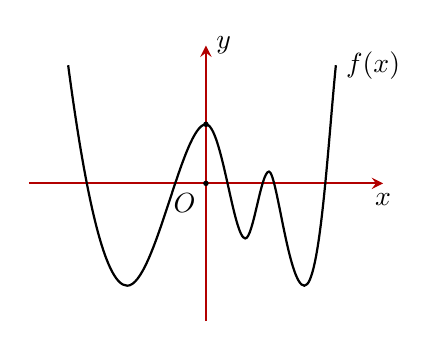
\begin{tikzpicture}[>=stealth, thick,scale=.5]
			\draw[->, red!70!black] (-4.5, 0) -- (4.5, 0) node[below, text=black] {$x$};
			\draw[->, red!70!black] (0, -3.5) -- (0, 3.5) node[right, text=black] {$y$};
			\fill (0,0) circle (2pt) node[below left] {$O$};
			\fill (0, 1.5) circle (2pt);
			\draw[thick]
			(-3.5, 3)
			.. controls (-3.1, 0) and (-2.6, -2.6) .. (-2, -2.6) % Đáy 1 bên trái
			.. controls (-1.3, -2.6) and (-0.6, 1.5) .. (0, 1.5) % Đỉnh 1 (trên trục Oy)
			.. controls (0.4, 1.5) and (0.7, -1.4) .. (1, -1.4) % Đáy 2
			.. controls (1.2, -1.4) and (1.4, 0.3) .. (1.6, 0.3) % Đỉnh 2 (nhỏ)
			.. controls (1.8, 0.3) and (2.1, -2.6) .. (2.5, -2.6) % Đáy 3
			.. controls (2.9, -2.6) and (3.1, 1) .. (3.3, 3) % Nhánh lên
			node[right, black] {$f (x)$};
	\end{tikzpicture}}
	\loigiai{
		Dựa vào đồ thị hàm số, ta có đồ thị có $3$ điểm cực tiểu; có $2$ điểm cực đại.\\
		Vậy tổng số điểm cực trị của hàm số là $5$.
	}
\end{ex}
%%%=============================%%%

%%%=============EX_6=============%%%
\begin{ex}%[2H2N2-3]%[TDMZZ03]%[Nguyễn Sơn Thành]
	Trong không gian $Oxyz$, cho hai điểm $A(2;0;-1)$, $B(-1;3;1)$. Tọa độ của vectơ $\overrightarrow{AB}$ tương ứng là
	\choice
	{$\left(3;-3;-2\right)$}
	{$\left(1;3;0\right)$}
	{$\left(3;-1;-2\right)$}
	{\True $\left(-3;3;2\right)$}
	\loigiai{
		Ta có tọa độ của vectơ $\overrightarrow{AB}=\left(-3;3;2\right)$.
	}
\end{ex}
%%%=============================%%%

%%%=============EX_7=============%%%
\begin{ex}%[2D4N1-2]%[TDMZZ03]%[Bồ Văn Hậu]
	Họ nguyên hàm của hàm số $f(x)=3x^4$ là
	\choice
	{$x^3+C$}
	{$x^5+C$}
	{\True $\dfrac{3}{5}x^5+C$}
	{$12x^3+C$}
	\loigiai{
		Với mọi $x\in \mathbb{R}$, ta có
		$\displaystyle\int 3x^4 \mathrm{\,d}x=3\cdot \dfrac{x^5}{5}+C=\dfrac{3}{5}x^5+C$.
	}
\end{ex}
%%%=============================%%%

%%%=============EX_8=============%%%
\begin{ex}%[2H5H2-5]%[TDMZZ03]%[Lê Phúc]
	Trong không gian $Oxyz$, cho đường thẳng $d\colon \dfrac{x-1}{2}=\dfrac{y+2}{3}=\dfrac{z-1}{-1}$. Giao điểm của đường thẳng $d$ và mặt phẳng tọa độ $(Oxy)$ tương ứng là
	\choice
	{$(1;-2;1)$}
	{\True $(3;1;0)$}
	{$(3;2;0)$}
	{$(2;3;-2)$}
	\loigiai{
		Đường thẳng $d$ được viết lại dưới dạng tham số là $d\colon \heva{&x=1+2t\\&y=-2+3t\\&z=1-t.}$\\
		Gọi $M=d\cap (Oxy)$.\\
		Ta có $M\in d\Rightarrow M(1+2t;-2+3t;1-t)$.\\
		Mặt khác $M\in (Oxy)\colon z=0$ nên
		\[1-t=0\Leftrightarrow t=1.\]
		Suy ra $M(3;1;0)$.
	}
\end{ex}
%%%=============================%%%

%%%=============EX_9=============%%%
\begin{ex}%[2D1N5-1]%[TDMZZ03]%[Trần Văn Thiện]
	\immini[thm]{Hỏi đồ thị ở hình bên là của hàm số nào cho dưới đây
		\choice
		{$y=\dfrac{ax^2+bx+c}{mx+n}$}
		{$y=\dfrac{ax+b}{cx+d}$}
		{ $y=-x^3+bx^2+cx+d$}
		{\True $y=x^3+bx^2+cx+d$}
	}
	{
		%3) Đồ thị hàm số bậc Ba y=ax^3+bx^2+cx+d ====================================
		\begin{tikzpicture} [>=stealth, line join=round, line cap=round, scale=0.6]
			\def\xmin{-4};\def\ymin{-2};\def\xmax{4};\def\ymax{4};
			\coordinate (O) at (0,0);
			\draw[->] (\xmin,0)--(\xmax,0) node[below]{$x$};
			\draw[->] (0,\ymin)--(0,\ymax) node[left]{$y$};
			\fill (O) node[below left]{$O$} circle(1pt);
			\clip ({\xmin+0.1},{\ymin+0.1}) rectangle ({\xmax-0.1},{\ymax-0.1});
			\draw[samples=100] plot[domain=-2.2:2.1](\x,{1*(\x)^3-3*(\x)+1});
	\end{tikzpicture} 	}
	\loigiai{
		Đồ thị đã cho là đồ thị của hàm số đa thức bậc ba $y=ax^3+bx^2+cx+d$ với hệ số $a>0$.
	}
\end{ex}
%%%=============================%%%

%%%=============EX_10=============%%%
\begin{ex}%[2D3H1-4]%[TDMZZ03]%[Đình Nguyên]
	Cho một mẫu số liệu ghép nhóm $M$ có đầu mút phải của nhóm thứ nhất bằng $5$ và đầu mút trái của nhóm cuối cùng bằng $20$. Biết các nhóm có độ dài bằng nhau và khoảng biến thiên bằng $21$. Phần tử đại diện của nhóm thứ ba của $M$ bằng
	\choice
	{$8$}
	{$9$}
	{$\dfrac{21}{2}$}
	{\True $\dfrac{19}{2}$}
	\loigiai{
		Gọi độ dài mỗi nhóm là $h$. Giả sử mẫu số liệu có $k$ nhóm.\\
		Đầu mút trái của nhóm đầu tiên là $a_1$, đầu mút phải của nhóm cuối cùng là $a_{k+1}$.\\
		Ta có đầu mút phải nhóm $1$ là $a_2 = 5 \Rightarrow a_1 = 5 - h$.\\
		Đầu mút trái nhóm cuối là $a_k = 20 \Rightarrow a_{k+1} = 20 + h$.\\
		Khoảng biến thiên $R = a_{k+1} - a_1 = (20 + h) - (5 - h) = 15 + 2h = 21 \Rightarrow h = 3$.\\
		Nhóm thứ ba là $[a_3; a_4) = [a_2 + h; a_2 + 2h) = [5 + 3; 5 + 6) = [8; 11]$.\\
		Giá trị đại diện nhóm thứ ba là $\dfrac{8 + 11}{2} = \dfrac{19}{2}$.
	}
\end{ex}
%%%=============================%%%

%%%=============EX_11=============%%%
\begin{ex}%[2D4H2-2]%[TDMZZ03]%[Huỳnh Quốc Đạt]
	Biết rằng $\displaystyle\int\limits_{0}^1f(x)\mathrm{\,d}x=2$. Giá trị của tích phân $\displaystyle\int\limits_{0}^1\left[f(x)-2x\right]\mathrm{\,d}x$ bằng
	\choice
	{\True $1$}
	{$0$}
	{$2$}
	{$3$}
	\loigiai{
		Ta có	$\displaystyle\int\limits_{0}^1\left[f(x)-2x\right]\mathrm{\,d}x$=$\displaystyle\int\limits_{0}^1f(x)\mathrm{\,d}x-\displaystyle\int\limits_{0}^1 2x\mathrm{\,d}x=2-1=1$.}
\end{ex}
%%%=============================%%%

%%%=============EX_12=============%%%
\begin{ex}%[2H2H2-4]%[TDMZZ03]%[Nguyễn Trí Minh Tuấn]
	Cho hình chóp tứ giác đều $S. ABCD$ có mặt bên là tam giác đều có cạnh bằng $4$. Giá trị của $\left(\overrightarrow{SA}+\overrightarrow{SB}+\overrightarrow{SC}\right)\cdot \overrightarrow{AD}$ bằng
	\choice
	{$0$}
	{$8\sqrt{3}$}
	{\True $-8$}
	{$16$}
	\loigiai{
		\immini{
			Gọi $O$ là tâm đáy $ABCD$. Ta có
			\[
			\overrightarrow{SA}=\overrightarrow{SO}+\overrightarrow{OA},\quad
			\overrightarrow{SB}=\overrightarrow{SO}+\overrightarrow{OB},\quad
			\overrightarrow{SC}=\overrightarrow{SO}+\overrightarrow{OC}.
			\]
			Suy ra
			\allowdisplaybreaks
			\begin{eqnarray*}
				\left(\overrightarrow{SA}+\overrightarrow{SB}+\overrightarrow{SC}\right)\cdot \overrightarrow{AD}
				&=&\left(3\overrightarrow{SO}+\overrightarrow{OA}+\overrightarrow{OB}+\overrightarrow{OC}\right)\cdot \overrightarrow{AD}\\
				&=&\left(3\overrightarrow{SO}+\overrightarrow{OB}\right)\cdot \overrightarrow{AD}.
			\end{eqnarray*}
			Lại có $SO\perp (ABCD)$ nên $\overrightarrow{SO}\perp \overrightarrow{AD}$ hay $\overrightarrow{SO}\cdot \overrightarrow{AD}=0$, suy ra
			\[
			\left(\overrightarrow{SA}+\overrightarrow{SB}+\overrightarrow{SC}\right)\cdot \overrightarrow{AD}
			=\overrightarrow{OB}\cdot \overrightarrow{AD}=\dfrac{1}{2}\overrightarrow{DB}\cdot \overrightarrow{AD}=\left(\dfrac{1}{2}\overrightarrow{AB}-\dfrac{1}{2}\overrightarrow{AD}\right)\cdot \overrightarrow{AD}=\dfrac{1}{2}\overrightarrow{AB}\cdot \overrightarrow{AD}-\dfrac{1}{2}\overrightarrow{AD}^2
			=0-\dfrac{1}{2}\cdot 16=-8.
			\]
			Vậy
			$\left(\overrightarrow{SA}+\overrightarrow{SB}+\overrightarrow{SC}\right)\cdot \overrightarrow{AD}=-8$.
		}
		{
			\begin{tikzpicture}[line cap=round, line join=round,>=stealth,font=\footnotesize,scale=0.8]
				\path 
				coordinate (A) at (0,0)
				coordinate (B) at (-2.5,-2.5)
				coordinate (D) at (5,0)
				coordinate (C) at ($(B)+(D)-(A)$)
				coordinate (O) at ($(B)!.5!(D)$)
				coordinate (S) at ($(O)+(0,5)$)
				;
				\draw (B)--(C)--(D) (S)--(B) (S)--(D) (S)--(C);
				\draw[dashed] (B)--(A)--(D)--(B) (A)--(C) (S)--(A) (S)--(O);
				\foreach \x/\g in {A/left, B/above left, C/right,D/right, O/below, S/above right}
				{
					\draw[fill=black] (\x) circle (1pt) node[\g] {$\x$} ;
				}
			\end{tikzpicture}
		}
	}
\end{ex}
%%%=============================%%%
\Closesolutionfile{ans}

\cauds
\Opensolutionfile{ans}[ans/ansTN-DungSai]
%%%=============EX_13=============%%%
\begin{ex}%[2D4H3-1]%[TDMZZ03]%[Văn Minh Thoại]
	Cho hàm số $y=f(x)=x^4-8x^2$ có đồ thị $(C)$.
	\choiceTF
	{\True Hàm số $f(x)$ nghịch biến trên các khoảng $(-\infty;-2)$; $(0;2)$}
	{\True $(C)$ có đúng một điểm cực đại}
	{\True Các điểm cực trị của $(C)$ tạo thành một tam giác có diện tích bằng $32$}
	{Diện tích hình phẳng giới hạn bởi $(C)$ và trục hoành là $24{,}1$ (đơn vị diện tích) \textit{(làm tròn kết quả đến hàng phần mười)}}
	\loigiai{
		Ta có $y=f(x)=x^4-8x^2$, suy ra $y'=4x^3-16x$. \\
		Xét phương trình $y'=0\Leftrightarrow4x^3-16x=0\Leftrightarrow\hoac{&x=0\\&x=2\\&x=-2.}$\\
		Bảng biến thiên
		\begin{center}
			
\begin{tikzpicture}
				\tkzTabInit[nocadre=false,lgt=1.2,espcl=2.5]{$x$ /0.6, $y'$ /0.6, $y$ /2}
				{$-\infty$,$-2$,$0$,$2$,$+\infty$}
				\tkzTabLine{,-,0,+,0,-,0,+,}
				\tkzTabVar{+/$+\infty$, -/$-16$, +/$0$, -/$-16$, +/$+\infty$}
			\end{tikzpicture}
		\end{center}
		\begin{itemchoice}
			\itemch Dựa vào bảng biến thiên, ta thấy hàm số nghịch biến trên các khoảng $(-\infty;-2)$ và $(0;2)$.
			\itemch Dựa vào bảng biến thiên, ta thấy hàm số đạt cực đại tại $x=0$.\\
			Vậy đồ thị $(C)$ có đúng một điểm cực đại.
			\itemch Đồ thị $(C)$ hàm số $y=f(x)=x^4-8x^2$ là
			\begin{center}
				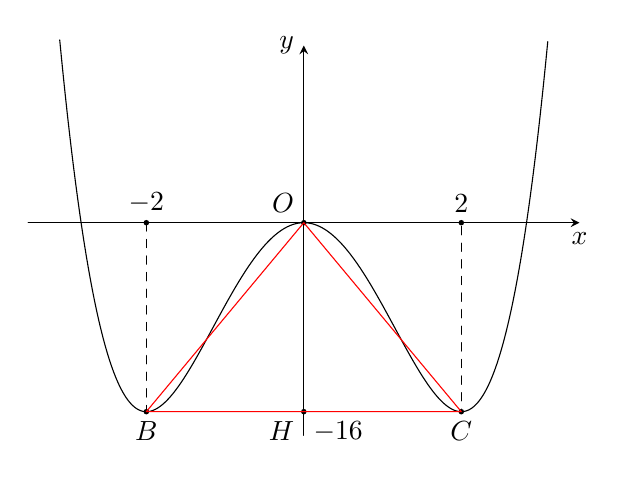
\begin{tikzpicture}[x=1cm,y=0.15cm,declare function={f (\x)=(\x)^4-8*(\x)^2;},line join=round,line cap=round,>=stealth,scale=1]
					\draw[->] (-3.5,0) -- (3.5,0) node[below] {$x$};
					\draw[->] (0,-18) -- (0,15) node[left] {$y$};
					\node at (0,0) [above left] {$O$};
					\draw[smooth,domain=-3.1:3.1,samples=500] plot (\x,{f (\x)});
					\draw[dashed] (-2,0) node[above]{$-2$}-- (-2,-16) -- (2,-16) -- (2,0) node[above]{$2$};
					\draw[dashed] (0,-16) node[below right]{$-16$};
					\fill (0,0) circle (1pt)
					(-2,0) circle (1pt)
					(2,0) circle (1pt)
					(-2,-16) circle (1pt)
					(2,-16) circle (1pt)
					(0,-16) circle (1pt);
					\node[below] at (-2,-16) {$B$};
					\node[below] at (2,-16) {$C$};
					\node[below left] at (0,-16) {$H$};
					\draw[red] (0,0)--(-2,-16)--(2,-16)--cycle;
				\end{tikzpicture}
			\end{center}
			Tọa độ các điểm cực trị của đồ thị hàm số là $O(0;0)$, $B(2;-16)$, $C(-2;-16)$.\\
			Tam giác $OBC$ cân tại $O$. Gọi $H$ là trung điểm của $BC$, ta được $H(0;-16)$.\\
			Độ dài đường cao $OH=16$, độ dài đáy $BC=4$.\\
			Diện tích tam giác $OBC$ là $S_{\triangle OBC}=\dfrac{1}{2}OH\cdot BC=\dfrac{1}{2}\cdot16\cdot4=32$.
			\itemch Phương trình hoành độ giao điểm của $(C)$ và trục hoành là
			\[x^4-8x^2=0\Leftrightarrow\hoac{&x=0\\&x=2\sqrt{2}\\&x=-2\sqrt{2}.}\]
			Diện tích hình phẳng giới hạn bởi $(C)$ và trục hoành là
			\[S=\displaystyle\int\limits_{-2\sqrt{2}}^{2\sqrt{2}}\left|x^4-8x^2\right|\mathrm{\,d}x=2\displaystyle\int\limits_{0}^{2\sqrt{2}}\left(8x^2-x^4\right)\mathrm{\,d}x=\left.2\cdot\left(\dfrac{8x^3}{3}-\dfrac{x^5}{5}\right)\right|_{0}^{2\sqrt{2}}=\dfrac{512\sqrt{2}}{15}\approx48{,}3.\]
		\end{itemchoice}
	}
\end{ex}
%%%=============================%%%

%%%=============EX_14=============%%%
\begin{ex}%[2D4H3-4]%[TDMZZ03]%[Dương Công Tạo]
	Cho một vật thể nằm dọc theo trục $Ox$, được giới hạn bởi hai mặt phẳng vuông góc với trục $Ox$ tại hai điểm có hoành độ $x_1 = 1$, $x_2 = 5$. Dùng một mặt phẳng $(\alpha)$ vuông góc với trục $Ox$ tại điểm có hoành độ $x \in [1;5]$ thì cho ta thiết diện là một hình
	vuông có cạnh bằng $4-x$ nếu $x \le 3$, còn khi $x > 3$ thì lại cho ta thiết diện là một hình vuông có cạnh bằng $\dfrac{x-1}{2}$. Gọi $S(x)$ là diện tích của thiết diện khi cắt vật thể bởi $(\alpha)$.
	\choiceTF
	{$S(x)=(x-3)^2$ với mọi $x \in [1;5]$}
	{\True $S(x)$ là một hàm số liên tục trên đoạn $[1;5]$}
	{Thể tích của vật thể bằng $5{,}33$ (\textit{làm tròn kết quả đến hàng phần trăm})}
	{Dùng một mặt phẳng vuông góc với trục $Ox$ tại điểm có hoành độ $x = b$ để chia vật thể thành hai phần có thể tích bằng nhau. Khi đó $b = 2{,}4$}
	\loigiai{
		\begin{itemchoice}
			\itemch
			\begin{itemize}
				\item Trên đoạn $[1;3]$, ta có $S(x)=(4-x)^2$.
				\item Trên đoạn $[3;5]$, ta có $S(x)=\left(\dfrac{x-1}{2}\right)^2$.
			\end{itemize}
			% Do đó, diện tích của thiết diện khi cắt vật thể bởi $(\alpha)$ là $S(x)=(4-x)^2+\left(\dfrac{x-1}{2}\right)^2$.
			Do đó, mệnh đề $S(x)=(x-3)^2$ với mọi $x \in [1;5]$ là sai.
			\itemch Ta có $S(x)=\heva{&(4-x)^2&\text{khi }1\leq x\leq 3\\&\dfrac{1}{4}(x-1)^2&\text{khi }3<x\leq 5.}$\\
			\begin{itemize}
				\item Với $1\leq x< 3$, ta có $S(x)=(4-x)^2$ liên tục trên nửa khoảng $[1;3)$.\quad$(1)$
				\item Với $3<x\leq 5$, ta có $S(x)=\dfrac{1}{4}(x-1)^2$ liên tục trên nửa khoảng $(3;5]$.\quad$(2)$
				\item Tại $x=3$, ta có
				\begin{itemize}
					\item[\faCheckCircleO] $S(3)=(4-3)^2=1$.
					\item[\faCheckCircleO] $\lim\limits_{x\to 3^-}S(x)=\lim\limits_{x\to 3^-}(4-x)^2=1$.
					\item[\faCheckCircleO] $\lim\limits_{x\to 3^+}S(x)=\lim\limits_{x\to 3^+}\dfrac{1}{4}(x-1)^2=1$.\\
					Vì $S(3)=\lim\limits_{x\to 3^-}S(x)=\lim\limits_{x\to 3^+}S(x)=1$ nên $S(x)$ liên tục tại $x=3$.\quad$(3)$
				\end{itemize}
				Từ $(1)$, $(2)$ và $(3)$ suy ra $S(x)$ liên tục trên đoạn $[1;5]$.
			\end{itemize}
			\itemch Thể tích của vật thể là \[V=\displaystyle\int\limits_1^3(4-x)^2\mathrm{\,d}x+\dfrac{1}{4}\displaystyle\int\limits_3^5(x-1)^2\mathrm{\,d}x=\dfrac{40}{3}\approx 13{,}33.\]
			\itemch Gọi $V_1$ là thể tích phần bên trái mặt phẳng.\\
			Ta có $\displaystyle\int\limits_1^3(4-x)^2\mathrm{\,d}x = \dfrac{26}{3} > \dfrac{V}{2}$ nên $b < 3$.\\
			Khi đó, theo giả thiết, ta có \allowdisplaybreaks
			\begin{eqnarray*}
				V_1=\dfrac{1}{2}V&\Leftrightarrow& \displaystyle\int\limits_1^b(4-x)^2\mathrm{\,d}x=\dfrac{1}{2}\cdot\dfrac{40}{3}\\
				&\Leftrightarrow& \big.-\dfrac{1}{3}(4-x)^3\bigg|_1^b=\dfrac{20}{3}\\
				&\Leftrightarrow& -\dfrac{1}{3}\left((4-b)^3-27\right)=\dfrac{20}{3}\\
				&\Leftrightarrow& b\approx 2{,}09.
			\end{eqnarray*}
		\end{itemchoice}
	}
\end{ex}
%%%=============================%%%

%%%=============EX_15=============%%%
\begin{ex}%[2H2V1-4]%[TDMZZ03]%[Nguyễn Văn Sang]
	\immini[thm]{Trong không gian, cho bốn sợi dây buộc với nhau tại điểm $I$.
		Sợi dây được cân bằng bởi $4$ lực dọc theo $4$ sợi dây thứ $1$, thứ $2$, thứ $3$, thứ $4$ lần lượt là $\overrightarrow{F}_1$, $\overrightarrow{F}_2$, $\overrightarrow{F}_3$, $\overrightarrow{F}_4$.
		Biết rằng $\left|\overrightarrow{F}_1\right|=180$ N, $\left|\overrightarrow{F}_3\right|=220$ N,
		$\left(\overrightarrow{F}_2,\overrightarrow{F}_4\right)=120^\circ$,
		$\left(\overrightarrow{F}_1,\overrightarrow{F}_3\right)=50^\circ$.
		Trong bài toán đơn vị lực tính theo Newton (N).}{
		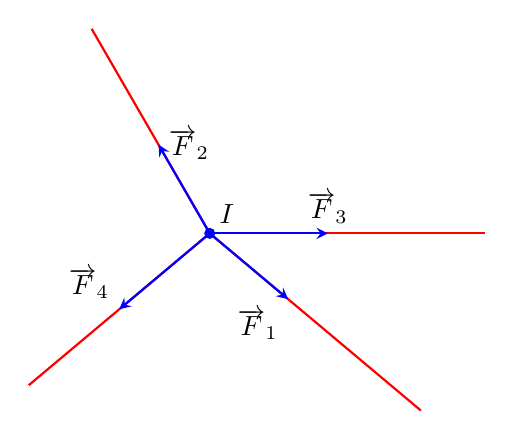
\begin{tikzpicture}[>=stealth, scale=1]
			\coordinate (I) at (0,0);
			
			% Sợi dây (đường màu đỏ)
			\draw[red, thick] (I) -- (0:3.5);
			\draw[red, thick] (I) -- (-40:3.5);
			\draw[red, thick] (I) -- (120:3);
			\draw[red, thick] (I) -- (220:3);
			
			% Lực (vector màu xanh)
			\draw[->, blue, thick] (I) -- (0:1.5) node[above, text=black] {$\overrightarrow{F}_3$};
			\draw[->, blue, thick] (I) -- (-40:1.3) node[below left, text=black] {$\overrightarrow{F}_1$};
			\draw[->, blue, thick] (I) -- (120:1.3) node[right, text=black] {$\overrightarrow{F}_2$};
			\draw[->, blue, thick] (I) -- (220:1.5) node[above left, text=black] {$\overrightarrow{F}_4$};
			
			% Điểm I
			\fill[blue] (I) circle (2pt) node[above right, text=black] {$I$};
		\end{tikzpicture}
	}
	\choiceTF
	{\True $\overrightarrow{F}_1+\overrightarrow{F}_2+\overrightarrow{F}_3+\overrightarrow{F}_4=\overrightarrow{0}$}
	{\True $\left|\overrightarrow{F}_2+\overrightarrow{F}_4\right|=363$ N \textit{(làm tròn kết quả đến hàng đơn vị)}}
	{Nếu $\left|\overrightarrow{F}_2\right|=180$ N thì $\left|\overrightarrow{F}_4\right|=315$ N \textit{(làm tròn kết quả đến hàng đơn vị)}}
	{\True $\left|\overrightarrow{F}_4\right|$ đạt giá trị lớn nhất bằng $419$ N \textit{(làm tròn kết quả đến hàng đơn vị)}}
	\loigiai{
		Vì sợi dây cân bằng tại $I$ nên
		$$\overrightarrow{F}_1+\overrightarrow{F}_2+\overrightarrow{F}_3+\overrightarrow{F}_4=\overrightarrow{0}.$$
		Do đó $\overrightarrow{F}_2+\overrightarrow{F}_4=-\left(\overrightarrow{F}_1+\overrightarrow{F}_3\right)$, suy ra
		$\left|\overrightarrow{F}_2+\overrightarrow{F}_4\right|=\left|\overrightarrow{F}_1+\overrightarrow{F}_3\right|$.
		\begin{itemchoice}
			\itemch Điều kiện cân bằng $$\overrightarrow{F}_1+\overrightarrow{F}_2+\overrightarrow{F}_3+\overrightarrow{F}_4=\overrightarrow{0}.$$
			\itemch Ta có
			\allowdisplaybreaks
			\begin{align*}
				\left|\overrightarrow{F}_1+\overrightarrow{F}_3\right|^2
				&= \left|\overrightarrow{F}_1\right|^2 + \left|\overrightarrow{F}_3\right|^2 + 2\left|\overrightarrow{F}_1\right|\left|\overrightarrow{F}_3\right|\cos 50^\circ\\
				&= 180^2 + 220^2 + 2 \cdot 180 \cdot 220 \cdot \cos 50^\circ\\
				&\approx 32400 + 48400 + 50879 = 131679.
			\end{align*}
			Vậy $\left|\overrightarrow{F}_2+\overrightarrow{F}_4\right| = \sqrt{131679} \approx 363$ N.
			\itemch Đặt $\left|\overrightarrow{F}_4\right|=y$. Vì $\left(\overrightarrow{F}_2,\overrightarrow{F}_4\right)=120^\circ$ nên
			$$\left|\overrightarrow{F}_2+\overrightarrow{F}_4\right|^2 = 180^2 + y^2 + 2\cdot 180\cdot y\cdot\cos 120^\circ \approx 131679.$$
			Suy ra $y^2 - 180y + 32400 - 131679 = 0 \Leftrightarrow \hoac{& y \approx 418\,\text{N} &\text{(nhận)}\\& y \approx -238\,\text{N} &\text{(loại).}}$\\
			Vậy $\left|\overrightarrow{F}_4\right| \approx 418$ N.
			\itemch Đặt $\left|\overrightarrow{F}_2\right|=x$, $\left|\overrightarrow{F}_4\right|=y$. Ta có
			$x^2 + y^2 - xy = 363^2 $ vì $\cos120^\circ=-\dfrac{1}{2}$.\\
			Ta có phương trình bậc hai ẩn $x$
			$$x^2 - y \cdot x + \left(y^2 - 363^2\right) = 0.$$
			Để tồn tại $x$, ta phải có $\Delta \ge 0$
			$$\Delta = y^2 - 4\left(y^2 - 363^2\right) \ge 0 \Rightarrow 3y^2 \le 4 \cdot 363^2 \Rightarrow y^2 \le \dfrac{4}{3} \cdot 363^2 \Rightarrow y \le \dfrac{2\cdot 363}{\sqrt{3}} \approx 419\,\text{N}.$$
			Vậy $y_{\max} \approx 419$ N (đạt được khi $x = \dfrac{y}{2} = \dfrac{363}{\sqrt{3}}$).
		\end{itemchoice}
	}
\end{ex}
%%%=============================%%%

%%%=============EX_16=============%%%
\begin{ex}%[2D6V2-4]%[TDMZZ03]%[Vũ Hồng Toàn]
	Bạn Hùng hằng ngày đi học bằng xe đạp hoặc bằng xe buýt với tỉ lệ đi học muộn của các phương tiện khi được sử dụng lần lượt là $15\%$ và $30\%$. Ngày thứ hai (Monday) bạn Hùng chọn đi xe đạp tới trường, các ngày sau đó bạn ấy sẽ chọn phương tiện theo quy tắc: nếu hôm trước không đi muộn thì sẽ giữ nguyên phương tiện để đi hôm sau, còn nếu hôm trước đi muộn thì sẽ đổi phương tiện để đi hôm sau. Gọi $A$, $B$, $C$ lần lượt là các biến cố bạn Hùng đi học muộn ngày thứ hai, thứ ba, thứ tư.
	\choiceTF
	{\True $\mathrm{P}(A) = 0{,}15$; $\mathrm{P}\left(\overline{A}\right) = 0{,}85$}
	{$\mathrm{P}(B) = 0{,}22$}
	{$\mathrm{P}(A|B) = 0{,}35$}
	{$\mathrm{P}(C) = \dfrac{29}{200}$}
	\loigiai{
		\begin{itemize}
			\item Gọi $X$ là phương tiện xe đạp.
			\item Thứ hai (Monday): Hùng đi xe đạp.
		\end{itemize}
		Từ giả thiết, ta có sơ đồ cây như sau
		\begin{center}
			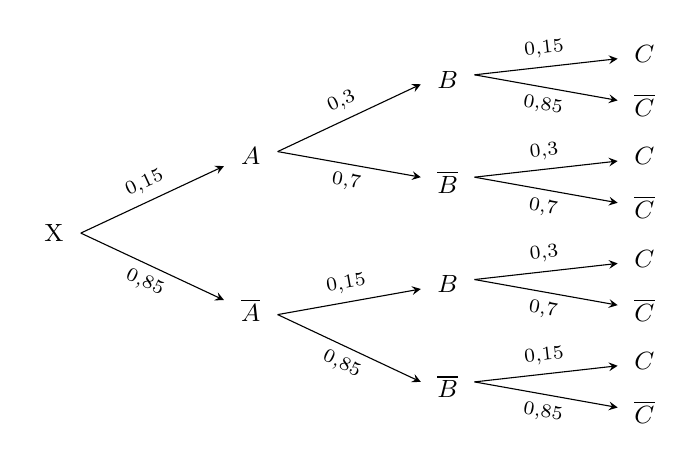
\begin{tikzpicture}[declare function={dai=2.5;cao=0.65;},>=stealth,font=\scriptsize]
				\tikzset{nhan/.style={minimum size=19pt,font=\small,inner sep=0pt}}
				\path (0,0) node[nhan] (G){\text{X}}
				% Tầng 1: Thứ hai (A)
				(dai,{1.5*cao}) node[nhan] (B) {$A$}
				(dai,{-1.5*cao}) node[nhan] (nB) {$\overline{A}$}
				% Tầng 2: Thứ ba (B)
				({2*dai},{3*cao}) node[nhan] (BA) {$B$}
				({2*dai},{cao}) node[nhan] (BnA) {$\overline{B}$}
				({2*dai},{-cao}) node[nhan] (nBA) {$B$}
				({2*dai},{-3*cao}) node[nhan] (nBnA) {$\overline{B}$}
				% Tầng 3: Thứ tư (C)
				({3*dai},{3.5*cao}) node[nhan] (C1) {$C$}
				({3*dai},{2.5*cao}) node[nhan] (nC1) {$\overline{C}$}
				({3*dai},{1.5*cao}) node[nhan] (C2) {$C$}
				({3*dai},{0.5*cao}) node[nhan] (nC2) {$\overline{C}$}
				({3*dai},{-0.5*cao}) node[nhan] (C3) {$C$}
				({3*dai},{-1.5*cao}) node[nhan] (nC3) {$\overline{C}$}
				({3*dai},{-2.5*cao}) node[nhan] (C4) {$C$}
				({3*dai},{-3.5*cao}) node[nhan] (nC4) {$\overline{C}$};
				
				% --- Vẽ mũi tên và ghi xác suất ---
				% Từ Gốc sang Thứ hai
				\draw[->] (G.0)--(B.200) node[sloped,pos=0.5,above]{$0{,}15$};
				\draw[->] (G.0)--(nB.160) node[sloped,pos=0.5,below]{$0{,}85$};
				
				% Từ Thứ hai sang Thứ ba
				\draw[->] (B.10)--(BA.190) node[sloped,pos=0.5,above]{$0{,}3$};
				\draw[->] (B.10)--(BnA.170) node[sloped,pos=0.5,below]{$0{,}7$};
				\draw[->] (nB.-10)--(nBA.190) node[sloped,pos=0.5,above]{$0{,}15$};
				\draw[->] (nB.-10)--(nBnA.170) node[sloped,pos=0.5,below]{$0{,}85$};
				
				% Từ Thứ ba sang Thứ tư (\mathrm{P}hần vẽ mới)
				% Nhánh 1: T3 muộn (đang đi Bus) -> T4 đổi sang Xe đạp (0.15)
				\draw[->] (BA.10)--(C1.190) node[sloped,pos=0.5,above]{$0{,}15$};
				\draw[->] (BA.10)--(nC1.170) node[sloped,pos=0.5,below]{$0{,}85$};
				
				% Nhánh 2: T3 không muộn (đang đi Bus) -> T4 giữ nguyên Bus (0.3)
				\draw[->] (BnA.10)--(C2.190) node[sloped,pos=0.5,above]{$0{,}3$};
				\draw[->] (BnA.10)--(nC2.170) node[sloped,pos=0.5,below]{$0{,}7$};
				
				% Nhánh 3: T3 muộn (đang đi Xe đạp) -> T4 đổi sang Bus (0.3)
				\draw[->] (nBA.10)--(C3.190) node[sloped,pos=0.5,above]{$0{,}3$};
				\draw[->] (nBA.10)--(nC3.170) node[sloped,pos=0.5,below]{$0{,}7$};
				
				% Nhánh 4: T3 không muộn (đang đi Xe đạp) -> T4 giữ nguyên Xe đạp (0.15)
				\draw[->] (nBnA.10)--(C4.190) node[sloped,pos=0.5,above]{$0{,}15$};
				\draw[->] (nBnA.10)--(nC4.170) node[sloped,pos=0.5,below]{$0{,}85$};
			\end{tikzpicture}
		\end{center}
		Quan sát sơ đồ cây, ta có
		\begin{itemchoice}
			\itemch $\mathrm{P}(A) = 0{,}15$ suy ra $\mathrm{P}\left(\overline{A}\right) =1-\mathrm{P}(A)=1-0{,}15= 0{,}85$.
			\itemch Áp dụng công thức xác suất toàn phần
			\begin{eqnarray*}
				\mathrm{P}(B)&=&\mathrm{P}(A)\cdot \mathrm{P}\left(B\mid A\right)+\mathrm{P}\left(\overline{A}\right)\cdot \mathrm{P}\left(B\mid \overline{A}\right)\\
				&=&0{,}15 \cdot 0{,}3 + 0{,}85 \cdot 0{,}15\\
				&=&0{,}1725.
			\end{eqnarray*}
			\itemch Áp dụng công thức xác suất có điều kiện
			\[\mathrm{P}(A|B) = \dfrac{\mathrm{P}(A \cap B)}{\mathrm{P}(B)}
			=\dfrac{0{,}15 \cdot 0{,}3}{0{,}1725}=0{,}2609.\]
			\itemch Ta có
			\allowdisplaybreaks
			\begin{eqnarray*}
				\mathrm{P}(C)&=&\mathrm{P}(A)\left(\mathrm{P}\left(B\mid A\right)\cdot \mathrm{P}\left(C\mid B\right)+\mathrm{P}\left(\overline{B}\mid A\right)\cdot \mathrm{P}\left(C\mid \overline{B}\right)\right)\\
				&&+\mathrm{P}\left(\overline{A}\right)\left(\mathrm{P}\left(B\mid \overline{A}\right)\cdot \mathrm{P}\left(C\mid B\right)+\mathrm{P}\left(\overline{B}\mid \overline{A}\right)\cdot \mathrm{P}\left(C\mid \overline{B}\right)\right)\\
				&=&0{,}15\cdot\left(0{,}3\cdot 0{,}15+0{,}7\cdot 0{,}3\right)+0{,}85\cdot\left(0{,}15\cdot 0{,}3+0{,}85\cdot 0{,}15\right)\\
				&=&\dfrac{1\,479}{8\,000}.
			\end{eqnarray*}
		\end{itemchoice}
	}
\end{ex}
%%%=============================%%%
\Closesolutionfile{ans}

\caukq
\Opensolutionfile{ans}[ans/ansTN-DienKhuyet]
%%%=============EX_17=============%%%
\begin{ex}%[1H8V5-4]%[TDMZZ03]%[Võ Hiệp]
	\immini[thm]{	Cho hình chóp cụt tứ giác đều $ABCD. A'B'C'D'$ có độ dài các cạnh $A'B'=4$, $AA'=6$, $AB=8$. Hãy tính khoảng cách giữa hai đường thẳng $AA'$ và $CD$ ({\it làm tròn kết quả đến hàng phần mười})?
	}{
		\begin{tikzpicture}[scale=.8,>=stealth, font=\footnotesize, line join=round, line cap=round]
			\def\a{4}
			\def\h{4}
			\path 	(0:0) coordinate (A)
			++(0:\a) coordinate (D)
			++(-130:\a/2) coordinate (C)
			($(A)+(C)-(D)$) coordinate (B)
			(intersection of A--C and B--D) coordinate (O)
			($(O)+(90:\h)$) coordinate (S)
			($(S)!.5!(A)$) coordinate (A')
			($(S)!.5!(B)$) coordinate (B')
			($(S)!.5!(C)$) coordinate (C')
			($(S)!.5!(D)$) coordinate (D')
			($(S)!.5!(O)$) coordinate (O')
			;
			\draw[dashed] (B)--(A)--(D) (A)--(A');
			\draw (A')--(B')--(C')--(D')--cycle (B)--(C)--(D) (B)--(B') (C)--(C') (D)--(D');
			\foreach \x/\g in {A/-60,B/-135,C/-45,D/45,A'/120,B'/150,C'/-10,D'/30}
			\fill[black] 	(\x) circle (1.5pt)
			($(\g:3mm)+(\x)$) node {$\x$};	
			%	\draw pic[draw,angle radius=3mm]{right angle=D--O--S};%Theo chiều dương	
		\end{tikzpicture}
	}
	\par
	\shortans[0]{7,5}
	\loigiai{
		\immini{
			Vì $ABCD. A'B'C'D'$ là hình chóp cụt đều nên ta có\\
			$\heva{&CD\parallel AB\\&AB\subset (ABB'AB)}\Rightarrow CD\parallel (ABB'A')$.\\
			Suy ra $\mathrm{d}(AA',CD)=\mathrm{d}\big(CD,(ABB'A')\big)=\mathrm{d}\big(D,(ABB'A')\big)$.\\
			Gọi $O$ và $O'$ lần lượt là tâm của hai hình vuông đáy. \\
			Ta có $\heva{&OO'\perp (ABCD)\\&OO'\subset (ACC'A')}\Rightarrow (ACC'A')\perp (ABCD)$.\\
			Gọi $H$ là hình chiếu vuông góc của $A'$ trên $(ABCD)$.\\
			Mà $(ACC'A')\cap (ABCD)=AC$.
		}{
			\begin{tikzpicture}[scale=.8,>=stealth, font=\footnotesize, line join=round, line cap=round]
				\def\a{4}
				\def\h{4.5}
				\path 	(0:0) coordinate (A)
				++(0:\a) coordinate (D)
				++(-145:\a/2) coordinate (C)
				($(A)+(C)-(D)$) coordinate (B)
				(intersection of A--C and B--D) coordinate (O)
				($(O)+(90:\h)$) coordinate (S)
				($(S)!.5!(A)$) coordinate (A')
				($(S)!.5!(B)$) coordinate (B')
				($(S)!.5!(C)$) coordinate (C')
				($(S)!.5!(D)$) coordinate (D')
				($(S)!.5!(O)$) coordinate (O')
				($(A')+(O)-(O')$) coordinate (H)
				($(A')+(A)-(H)$) coordinate (I)
				;
				\draw[dashed] (B)--(A)--(D) (A)--(A') (A)--(C)(O)--(O') (A')--(H)(A)--(I);
				\draw (A')--(B')--(C')--(D')--cycle (B)--(C)--(D) (B)--(B') (C)--(C') (D)--(D')  (A')--(C') --(I);
				\draw[->] (B)--++(-145:.7) node[right]{$x$};
				\draw[->] (D)--++(0:.7) node[below]{$y$};
				\draw[->] (I)--++(90:2) node[right]{$z$};
				\foreach \x/\g in {A/135,B/150,C/-45,D/45,A'/60,B'/150,C'/-10,D'/30,H/-90,O/-90,O'/20}
				\fill[black] 	(\x) circle (1.5pt)
				($(\g:3mm)+(\x)$) node {$\x$};	
				\draw pic[draw,angle radius=1.5mm]{right angle=A'--H--A};
				\draw pic[draw,angle radius=1.5mm]{right angle=O'--O--A};
			\end{tikzpicture}
		}
		\noindent
		Suy ra $H\in AC$ và $AH=\dfrac{AC-A'C'}{2}=\dfrac{8\sqrt{2}-4\sqrt{2}}{2}=2\sqrt{2}$.\\
		Tam giác $AHA'$ vuông tại $H$, suy ra $A'H = \sqrt{AA'^2 - AH^2} = \sqrt{6^2 - \left(2\sqrt{2}\right)^2} = 2\sqrt{7}$.\\
		Chọn hệ trục tọa độ $Axyz$, sao cho $B\in Ax$, $D\in Ay$, trục $Az$ hướng lên trên.
		Khi đó $A(0; 0; 0)$, $B(8; 0; 0)$, $D(0; 8; 0)$ và $H(2; 2; 0)$. Suy ra $A'\left(2; 2; 2\sqrt{7}\right)$.\\
		Ta có $\heva{&\overrightarrow{AB}=(8; 0; 0)\\& \overrightarrow{AA'}=\left(2; 2; 2\sqrt{7}\right)}\Rightarrow \left[\overrightarrow{AB}, \overrightarrow{AA'}\right]=\left(0, -16\sqrt{7}, 16\right)=-16\left(0, \sqrt{7}, -1\right)=-16\overrightarrow{n}$.\\
		Mặt phẳng $(ABB'A')$ đi qua $A$ và có vectơ pháp tuyến $\overrightarrow{n}$ có phương trình là $\sqrt{7}y-z=0$.\\
		Khoảng cách từ điểm $D(0; 8; 0)$ đến mặt phẳng $(ABB'A')$ là
		\[\mathrm{d} = \dfrac{\left|\sqrt{7} \cdot 8 + (-1) \cdot 0\right|}{\sqrt{\left(\sqrt{7}\right)^2 + (-1)^2}} = \dfrac{8\sqrt{7}}{\sqrt{7+1}} = 2\sqrt{14}.\]
		Vậy $\mathrm{d}(AA',CD)=\mathrm{d}\big(D,(ABB'A')\big)=2\sqrt{14}\approx 7{,}5$.
		
	}
\end{ex}
%%%=============================%%%

%%%=============EX_18=============%%%
\begin{ex}%[0D0C2-6]%[TDMZZ03]%[Lương Pho]
	Cho một đa giác đều có $16$ đỉnh nội tiếp một đường tròn có bán kính bằng $8$. Gọi $X$ là tập chứa tất cả các tứ giác có $4$ đỉnh là các đỉnh của đa giác đều đã cho. Chọn ngẫu nhiên từ $X$ một tứ giác. Gọi $p$ là xác suất để chọn được tứ giác có các cạnh lớn hơn $7$. Hãy tính $1\,000p$ (\textit{làm tròn kết quả đến hàng đơn vị})?
	\par
	\shortans[0]{77}
	\loigiai{
		\begin{itemize}
			\item Số phần tử của không gian mẫu (số tứ giác có thể tạo ra từ $16$ đỉnh) là
			$n(\Omega) = C_{16}^4 = 1\,820$.
			\item Gọi các đỉnh của đa giác đều là $A_1$, $A_2$, \ldots, $A_{16}$. \\
			Độ dài cạnh nối hai đỉnh $A_i$, $A_j$ cách nhau $k$ khoảng chia (cung nhỏ) được tính bởi công thức
			\[d = 2R \sin\dfrac{k\pi}{16} = 16 \sin\dfrac{k\pi}{16}.\]
			Để cạnh của tứ giác lớn hơn $7$, ta cần
			\[16 \sin\dfrac{k\pi}{16} > 7 \Leftrightarrow \sin\dfrac{k\pi}{16} > \dfrac{7}{16} \Rightarrow k \ge 3.\]
			Gọi $x_1$, $x_2$, $x_3$, $x_4$ là số cung nhỏ giữa các đỉnh liên tiếp của tứ giác theo thứ tự trên đa giác ($x_i \in \mathbb{Z}^+$).\\
			Ta có điều kiện
			$\heva{&x_1 + x_2 + x_3 + x_4 = 16 \\& x_i \ge 3.}$\\
			Đặt $y_i = x_i - 2 $. Khi đó
			\[\heva{&y_1 + y_2 + y_3 + y_4 = 8\\& y_i \ge 1.}\]
			Số nghiệm nguyên dương của phương trình này là $C_{8-1}^{4-1} = C_7^3 = 35$.\\
			Nếu cố định đỉnh bắt đầu thì có $16$ cách quay.\\
			Nhưng một tứ giác bị đếm $4$ lần (vì có $4$ đỉnh có thể làm điểm bắt đầu).\\
			Do đó $n(A) = \dfrac{16 \cdot 35}{4} = 140$.
			\item Xác suất cần tìm là
			$\mathrm{P}(A)=\dfrac{n(A)}{n(\Omega)}= \dfrac{140}{1\,820}=\dfrac{1}{13}$.\\
			Vậy $1\,000p = 1\,000 \cdot \dfrac{1}{13} \approx 77$.
		\end{itemize}
	}
\end{ex}
%%%=============================%%%

%%%=============EX_19=============%%%
\begin{ex}%[1D7C1-5]%[TDMZZ03]
	Có một khối lăng trụ tam giác như hình vẽ, có thiết diện là tam giác vuông $ABC$ có các cạnh là $AB = 260$ cm, $BC = 100$ cm, $CA = 240$ cm. Đỉnh $A$ di chuyển trên sàn nhà theo phương vuông góc với bức tường, đỉnh $B$ di chuyển trên tường theo phương vuông góc với sàn nhà. Biết rằng bức tường và sàn nhà vuông góc với nhau. Ở một thời điểm, khi mà đỉnh $A$ đang cách chân tường một đoạn bằng $150$ cm thì nó di chuyển với tốc độ bằng $v_A = 3{,}9$ cm/s thì tốc độ thay đổi của khoảng cách từ đỉnh $C$ đến sàn nhà bằng bao nhiêu cm/s (\textit{làm tròn kết quả đến hàng phần trăm})?
	\begin{center}
		\begin{tikzpicture}[scale=1,font=\footnotesize,line join=round,line cap=round,>=stealth]
			\def \a{8} \def \b{5} \def\g{15} \def \h{5}
			\path
			(0,0) coordinate (O)
			(180:\a) coordinate (O1)
			(\g:\b) coordinate (O3)
			($(O1)-(O)+(O3)$) coordinate (O2)
			($(O)+(90:\h)$) coordinate (O5)
			($(O3)+(90:\h)$) coordinate (O4)
			($(O)!.45!(O1)$) coordinate (A)
			++(60:3) coordinate (C)
			($(O)!.4!(O5)$) coordinate (B)
			(intersection of O2--O3 and A--C) coordinate (O2');
			\foreach \x in {A,B,C}{\path ($(\x)+(\g:\b)$) coordinate (\x');}
			\path
			(intersection of C--C' and O--O5) coordinate (C1)
			(intersection of A--A' and O--O5) coordinate (A1);
			\fill[cyan!40!gray!20] (O)--(O1)--(O2)--(O3)--cycle;
			\fill[brown!35] (A)--(B)--(C)--cycle;
			\fill[gray!25] (O)--(O3)--(O4)--(O5)--cycle;
			\fill[brown!27] (A)--(B)--(B')--(A')--cycle (B)--(C)--(C')--(B')--cycle;
			\fill[brown!30] (C)--(B)--(C1)--cycle (A)--(B)--(A1)--cycle;
			
			\draw (O1)--(O2)--(O2')
			(O3)--(O)--(O1)
			(O)--(O3)--(O4)--(O5)--cycle;
			\draw[thick] (A)--(B) node[midway,sloped,below]{$260$}--(C) node[midway,sloped,above]{$100$}--(A) node[pos=.4,left]{$240$}
			(C)--(C1)
			(A)--(A1);
			\draw[dashed,thick] (A1)--(A')--(B')--(C')--(C')--(C1)
			(B)--(B')
			(A')--(C');
			\draw[dashed] (O2')--(O3);
			\draw[->] (O)--($(A)+(180:0.75)$);
			\foreach \t/\g in {O/-90,A/-90,B/-45,C/135}{
				\fill (\t) circle (1pt) node[shift={(\g:7pt)}]{$\t$};}
			\foreach \x/\y/\z in {A/C/B,A/O/B} \draw pic[draw,angle radius=2mm]
			{right angle= \x--\y--\z};
			\node at ($(O1)+(6:2)$) {Sàn nhà};
			\path (O4)--(O5) node[midway,below=15pt,sloped]{Bức tường};
		\end{tikzpicture}
	\end{center}
	\par
	\shortans[0]{0,96}
	\loigiai{
		Chọn hệ trục tọa độ $Oxy$ như hình vẽ, với $O$ là chân tường, trục $Ox$ nằm trên sàn nhà và trục $Oy$ nằm trên bức tường.
		\immini{Tại thời điểm khảo sát, giả sử $A$ có tọa độ $(-x; 0)$ và $B$ có tọa độ $(0; y)$ với $x$, $y > 0$.\\
			Theo giả thiết, $AB = 260$ cm, áp dụng định lý Pythagoras ta có
			\[x^2 + y^2 = 260^2 \Rightarrow y = \sqrt{260^2 - x^2}.\]
			Khi $x = 150$ cm, ta có $y = \sqrt{260^2 - 150^2} = 10\sqrt{451}$ cm.\\
			Lấy đạo hàm hai vế theo thời gian $t$
			\[2x \cdot \dfrac{\mathrm{d}x}{\mathrm{d}t} + 2y \cdot \dfrac{dy}{\mathrm{d}t} = 0 \Rightarrow \dfrac{dy}{\mathrm{d}t} = -\dfrac{x}{y} \cdot \dfrac{\mathrm{d}x}{\mathrm{d}t}.\]
			Với $\dfrac{\mathrm{d}x}{\mathrm{d}t} = v_A = 3{,}9\,\text{cm/s}$, ta có
			\[\dfrac{dy}{\mathrm{d}t} = -\dfrac{150}{10\sqrt{451}} \cdot 3{,}9 = -\dfrac{15 \cdot 3{,}9}{\sqrt{451}} \quad \text{cm/s}.\]}{
			\begin{tikzpicture}[scale=.8,line join=round, line cap=round, >=stealth, font=\footnotesize]
				\coordinate (O) at (0,0);
				\coordinate (A) at (-3,0);
				\coordinate (B) at (0,4.247);
				\coordinate (C) at (-1.94,4.68);
				\draw[red, thick] (-6,0) -- (0,0) node[below left] {Sàn nhà};
				\draw[red, thick] (0,0) -- (0,6) node[below right] {Bức tường};
				\fill[red] (O) circle (2pt) node[below right] {$O$};
				\filldraw[fill=green!30!black, draw=blue, thick] (A) -- (B) -- (C) -- cycle;
				%\draw[blue] (A) -- (B) -- (C) -- cycle;
				\node[below] at (A) {$A$};
				\node[right] at (B) {$B$};
				\node[above left] at (C) {$C$};
				\draw[<->] (A) -- node[above] {$150\,\text{cm}$} (O);
				\path (A) -- (B) node[midway, below, sloped] {$260\,\text{cm}$};
				\path (B) -- (C) node[midway, above] {$100\,\text{cm}$};
				\path (A) -- (C) node[midway, left] {$240\,\text{cm}$};
				\draw[->, red, very thick] (A) -- ++(-1.5,0) node[above] {$v_A = 3{,}9\,\text{cm/s}$};
				\draw (-0.2,0) -- (-0.2,0.2) -- (0,0.2);
			\end{tikzpicture}
		}\noindent
		Gọi $\alpha$ là góc hợp bởi $AB$ và sàn nhà, ta có $\cos \alpha = \dfrac{x}{260}$ và $\sin \alpha = \dfrac{y}{260}$.\\
		Xét tam giác vuông $ABC$ tại $C$, gọi $\beta = \widehat{BAC}$.\\
		Ta có $\cos \beta = \dfrac{AC}{AB} = \dfrac{240}{260} = \dfrac{12}{13}$ và $\sin \beta = \dfrac{BC}{AB} = \dfrac{100}{260} = \dfrac{5}{13}$.\\
		Khoảng cách từ $C$ đến sàn nhà là tung độ $y_C$ của điểm $C$. Từ hình vẽ, ta có
		\[y_C = AC \cdot \sin(\alpha + \beta) = 240(\sin \alpha \cos \beta + \cos \alpha \sin \beta).\]
		Thay các giá trị $\sin \alpha$, $\cos \alpha$, $\sin \beta$, $\cos \beta$ vào ta được
		\[y_C = 240 \left( \dfrac{y}{260} \cdot \dfrac{12}{13} + \dfrac{x}{260} \cdot \dfrac{5}{13} \right) = \dfrac{12}{169}(12y + 5x).\]
		Tốc độ thay đổi của khoảng cách từ $C$ đến sàn nhà là
		\[v_C = \left| \dfrac{dy_C}{\mathrm{d}t} \right| = \left| \dfrac{12}{169} \left( 12 \dfrac{dy}{\mathrm{d}t} + 5 \dfrac{\mathrm{d}x}{\mathrm{d}t} \right) \right|.\]
		Thay các giá trị đã biết vào biểu thức
		\[v_C = \left| \dfrac{12}{169} \left( 12 \cdot \left( -\dfrac{15 \cdot 3{,}9}{\sqrt{451}} \right) + 5 \cdot 3{,}9 \right) \right| = \dfrac{46{,}8}{169} \left| 5 - \dfrac{180}{\sqrt{451}} \right| \approx 0{,}96\,\,\text{cm/s}.\]
	}
\end{ex}
%%%=============================%%%

%%%=============EX_20=============%%%
\begin{ex}%[2H5V2-8]%[TDMZZ03]%[Nguyễn Đức Tuấn Anh]
	\immini[thm]{Trong không gian $Oxyz$ có đơn vị dài trên mỗi trục là $10$ mét, mặt đất là mặt phẳng $(Oxy)$ từ gốc toạ độ $O$ một vật được ném lên trên với vận tốc ban đầu $\overrightarrow{v} = (3;1;4)$ với đơn vị tốc độ là m/s. Biết quỹ đạo chuyển động là một đường parabol $(P)$ nằm trong mặt phẳng $(\alpha)$ vuông góc với mặt đất và đi qua gốc $O$. Giá của vectơ $\overrightarrow{v}$ tiếp tuyến với $(P)$ và nằm trong $(\alpha)$. Biết độ cao cực đại của vật là $80$ mét. Gọi $(a;b;c)$ là toạ độ của vật khi nó cách gốc một khoảng bằng $90$ mét. Hãy tính $(a+b+c)$ (\textit{làm tròn kết quả đến hàng phần chục})?}{
		\begin{tikzpicture}[scale=0.8, font=\footnotesize, line join=round, line cap=round, >=stealth]
			\draw[->] (0,0)coordinate (O) -- (-1.5,-1.5) node[below right, text=black] {$x$};
			\draw[->] (0,0) -- (5,0) node[below, text=black] {$y$};
			\draw[->] (0,0) -- (0,3) node[left, text=black] {$z$};
			\draw[->] (O) -- (1.5, -0.525)coordinate (A);
			\draw[dashed] (A)--($(O)!3!(A)$) node[below, text=black] {$t$};
			\draw[dashed, domain=0:3.5, samples=50]  (O) .. controls (65:4)  .. ($(O)!2!(A)$);
			\draw[->] (0,0) -- (0.4, 1.4) node[above, text=black] {$\vec{v}$};
			\filldraw[draw=blue](0,0) circle (1pt)node[left]{$O$} ;
	\end{tikzpicture}}
	\par
	\shortans[0]{14,5}
	\loigiai{
		Ta có $\overrightarrow{v} = (3;1;4)$ tiếp xúc với $(P)$ tại $O$, do đó hình chiếu của nó là $\overrightarrow{u} = (3;1;0)$ chính là vectơ chỉ phương của đường thẳng đó.\\
		Mà $(P)$ đi qua $(O)$ nên phương trình tham số của $(P)$ có dạng $ \heva{&x = 3t \\ &y = t\\&z = at^2 + bt}\,(t>0)$. \\
		Vectơ tiếp tuyến của $(P)$ tại $O$ là $\overrightarrow{u} = (x'(0); y'(0); z'(0)) = (3; 1; b)$.\\
		Vì $\overrightarrow{u}$ phải cùng phương với vectơ vận tốc ban đầu $\overrightarrow{v} = (3;1;4)$, ta suy ra $b = 4$.\\
		Do quỹ đạo là một bề lõm hướng xuống đất nên hệ số $a<0$. Đặt $a = -k$ $(k>0)$, ta có
		$z(t) = 4t - kt^2$.\\
		Phương trình tham số của quỹ đạo $(P)$ có dạng $\heva{&x=3t \\&y=t \\&z=4t-kt^2}$ (với $t>0$, $k>0$).\\
		Độ cao $z$ đạt giá trị lớn nhất khi $t=\dfrac{2}{k}$, khi đó $z = 4\left(\dfrac{2}{k}\right) - k\left(\dfrac{2}{k}\right)^2 = \dfrac{4}{k}$.\\
		Theo giả thiết, độ cao cực đại là $80$ mét, tương ứng với cao độ lớn nhất là $\dfrac{80}{10} = 8$ đơn vị.\\
		Do đó $\dfrac{4}{k} = 8 \Rightarrow k = 0{,}5$.\\
		Phương trình quỹ đạo $(P)$ là $\heva{&x=3t \\&y=t \\&z=4t-0{,}5t^2.}$\\
		Gọi $(a;b;c)$ là toạ độ của vật khi vật cách gốc toạ độ $90$ mét, tức là cách $O$ một khoảng bằng $9$ đơn vị.\\
		Ta có $a=3t$, $b=t$, $c=4t-0{,}5t^2$ và $a^2+b^2+c^2=9^2=81$.\\
		Thay vào phương trình, ta được
		\[(3t)^2 + t^2 + \left(4t-0{,}5t^2\right)^2 = 81 \Leftrightarrow t^4 - 16t^3 + 104t^2 - 324 = 0.\]
		Giải phương trình trên ta thu được nghiệm dương $t \approx 2{,}0774$.\\
		Vậy $a+b+c = 3t + t + 4t - 0{,}5t^2\approx 14{,}46$.
	}
\end{ex}
%%%=============================%%%

%%%=============EX_21=============%%%
\begin{ex}%[2D4V3-1]%[TDMZZ03]%[Lê Hồ Quang Minh]
	Cho hình vuông $ABCD$ có $AB = 60\sqrt{2}$ cm. Gọi $(H)$ là tập hợp các điểm $M$ nằm trong hình vuông $ABCD$ và thỏa mãn $\mathrm{d}\big(M,BD\big) - 20 \ge MC$. Hãy tính diện tích hình phẳng $(H)$ theo đơn vị centimét vuông \textit{(làm tròn kết quả đến hàng đơn vị).}
	\par
	\shortans[0]{350}
	\loigiai{
		\begin{center}
			\begin{tikzpicture}[scale=0.08, font=\footnotesize, line join=round, line cap=round, >=stealth]
				% Trục toạ độ
				\draw[->] (-50,0) -- (50,0) node[below] {$x$};
				\draw[->] (0,-10) -- (0,60) node[left] {$y$};
				\fill (0,0) circle (1.5pt) node[below left] {$O$};
				
				% Parabol
				\fill[pattern=north east lines, pattern color=gray!50] plot[domain=-16.568:16.568, samples=100] (\x, {\x*\x/80}) -- (0,20) -- cycle;
				\draw[domain=-45:45, smooth, samples=100, thick] plot (\x, {\x*\x/80}) node[right] {$(P)$};
				
				% Các đường thẳng CB, CD
				\draw[thick, blue] (-25, 45) -- (45, -25) node[right, black] {$CD$};
				\draw[thick, blue] (25, 45) -- (-45, -25) node[left, black] {$CB$};
				
				% Điểm C
				\fill (0,20) circle (1.5pt) node[right] {$C(0;20)$};
				
				% Giao điểm
				\fill (16.568, 3.431) circle (1.5pt);
				\fill (-16.568, 3.431) circle (1.5pt);
				\draw[dashed] (16.568, 3.431) -- (16.568, 0) node[below] {$x_N$};
				\draw[dashed] (-16.568, 3.431) -- (-16.568, 0);
			\end{tikzpicture}
		\end{center}
		Đường chéo của hình vuông $BD = AB\sqrt{2} = 60\sqrt{2}\cdot\sqrt{2} = 120$\,cm.\\
		Khoảng cách từ $C$ đến $BD$ là $\dfrac{BD}{2} = 60$\,cm.\\
		Gọi $\Delta$ là đường thẳng song song với $BD$, nằm trong nửa mặt phẳng bờ $BD$ chứa điểm $C$ sao cho $\mathrm{d}\big(\Delta, BD\big) = 20$\,cm.\\
		Khi đó khoảng cách từ $C$ đến $\Delta$ là $60 - 20 = 40$\,cm.\\
		Với mọi điểm $M$ nằm trong hình vuông và cùng phía với $C$ so với $\Delta$, ta có $\mathrm{d}\big(M, BD\big) = \mathrm{d}\big(M, \Delta\big) + 20$.\\
		Giả thiết $\mathrm{d}\big(M, BD\big) - 20 \ge MC \Leftrightarrow \mathrm{d}\big(M, \Delta\big) \ge MC$.\\
		Điều kiện này chứng tỏ $M$ nằm trong (hoặc trên) parabol $(P)$ có tiêu điểm là $C$ và đường chuẩn là $\Delta$. \\
		Chọn hệ trục toạ độ $Oxy$ có gốc $O$ là đỉnh của parabol $(P)$, trục $Oy$ đi qua $O$, $C$ và hướng từ $O$ đến $C$. Trục $Ox$ đi qua $O$ và vuông góc với $Oy$.\\
		Khoảng cách từ tiêu điểm đến đường chuẩn là $p = 40$. Suy ra $C(0; 20)$.\\
		Phương trình của parabol là $(P)\colon x^2 = 2py = 80y \Rightarrow y = \dfrac{x^2}{80}$.\\
		Trục $Oy$ trùng với đường chéo $AC$ của hình vuông. Các cạnh $CD$ và $CB$ tạo với $AC$ một góc $45^\circ$.\\
		Trong hệ toạ độ $Oxy$, đường thẳng $CD$ đi qua $C(0; 20)$ và có hệ số góc $\tan(-45^\circ) = -1$ nên có phương trình $y = -x + 20$.\\
		Hoành độ giao điểm của $(P)$ và đường thẳng $CD$ (với $x > 0$) là nghiệm của phương trình:
		\[ \dfrac{x^2}{80} = -x + 20 \Leftrightarrow x^2 + 80x - 1600 = 0 \Rightarrow x = 40\sqrt{2} - 40. \]
		Do tính đối xứng, diện tích hình phẳng $(H)$ là
		\[ S = 2\displaystyle\int\limits_0^{40\sqrt{2}-40} \left(-x + 20 - \dfrac{x^2}{80}\right) \mathrm{\,d}x. \]
		Ta có $\displaystyle\int \left(-x + 20 - \dfrac{x^2}{80}\right) \mathrm{\,d}x = -\dfrac{x^2}{2} + 20x - \dfrac{x^3}{240}$.\\
		Thay cận $x = 40\sqrt{2} - 40$, ta tính được $S = \dfrac{6400\sqrt{2} - 8000}{3} \approx 350{,}32 \text{ cm}^2$.\\
		Làm tròn đến hàng đơn vị, ta được $350$.
	}
\end{ex}
%%%=============================%%%

%%%=============EX_22=============%%%
\begin{ex}%[0D0C2-3]%[TDMZZ03]%[Nguyễn Thành Hậu]
	Dùng các tờ tiền có mệnh giá $10$ nghìn, $20$ nghìn, $50$ nghìn để làm tất cả các phong lì xì sao cho mỗi phong lì xì đều có 3 tờ tiền và mỗi phong lì xì có tổng số tiền khác với các phong lì xì còn lại. Chia ngẫu nhiên các phong lì xì cho 3 cặp vợ chồng sao cho mỗi người được đúng một phong lì xì. Gọi $p$ là xác suất để các cặp vợ chồng đều được tổng số tiền bằng nhau. Hãy tính $10^{5}p$ \textit{(làm tròn kết quả đến hàng đơn vị)}.
	\par
	\shortans[0]{413}
	\loigiai{
		Để thuận tiện, ta tính số tiền bằng đơn vị chục nghìn đồng. Các tổng số tiền có thể có trong một phong lì xì gồm 3 tờ tiền là:
		\begin{itemize}
			\item Loại 3 tờ giống nhau: $1+1+1=3$; $2+2+2=6$; $5+5+5=15$.
			\item Loại 2 tờ giống nhau: $1+1+2=4$; $1+1+5=7$; $2+2+1=5$; $2+2+5=9$; $5+5+1=11$; $5+5+2=12$.
			\item Loại 3 tờ khác nhau: $1+2+5=8$.
		\end{itemize}
		Tập hợp các tổng số tiền gồm $10$ giá trị: $T = \{3; 4; 5; 6; 7; 8; 9; 11; 12; 15\}$.\\
		Số phần tử của không gian mẫu (chia $10$ phong lì xì khác nhau cho $6$ người) là $n(\Omega) = \mathrm{A}_{10}^6 = 151\,200$.\\
		Gọi $A$ là biến cố: "Các cặp vợ chồng đều được tổng số tiền bằng nhau".\\
		Ta cần chọn ra $3$ cặp phong lì xì từ tập $T$ sao cho tổng 2 phần tử trong mỗi cặp đều bằng nhau và bằng một số $S$.\\
		Liệt kê số lượng cặp có cùng tổng $S$:
		\begin{itemize}
			\item $S=11$: có $3$ cặp $(3,8); (4,7); (5,6) \Rightarrow \mathrm{C}_3^3 = 1$ cách chọn 3 cặp.
			\item $S=12$: có $3$ cặp $(3,9); (4,8); (5,7) \Rightarrow \mathrm{C}_3^3 = 1$ cách chọn.
			\item $S=13$: có $3$ cặp $(4,9); (5,8); (6,7) \Rightarrow \mathrm{C}_3^3 = 1$ cách chọn.
			\item $S=14$: có $3$ cặp $(3,11); (5,9); (6,8) \Rightarrow \mathrm{C}_3^3 = 1$ cách chọn.
			\item $S=15$: có $4$ cặp $(3,12); (4,11); (6,9); (7,8) \Rightarrow \mathrm{C}_4^3 = 4$ cách chọn.
			\item $S=16$: có $3$ cặp $(4,12); (5,11); (7,9) \Rightarrow \mathrm{C}_3^3 = 1$ cách chọn.
			\item $S=17$: có $3$ cặp $(5,12); (6,11); (8,9) \Rightarrow \mathrm{C}_3^3 = 1$ cách chọn.
			\item $S=18$: có $3$ cặp $(3,15); (6,12); (7,11) \Rightarrow \mathrm{C}_3^3 = 1$ cách chọn.
			\item $S=19$: có $3$ cặp $(4,15); (7,12); (8,11) \Rightarrow \mathrm{C}_3^3 = 1$ cách chọn.
			\item $S=20$: có $3$ cặp $(5,15); (8,12); (9,11) \Rightarrow \mathrm{C}_3^3 = 1$ cách chọn.
		\end{itemize}
		Các tổng $S$ khác đều có ít hơn $3$ cặp nên không thỏa mãn.\\
		Số cách chọn ra 3 cặp phong lì xì thỏa mãn yêu cầu là: $9 \cdot \mathrm{C}_3^3 + \mathrm{C}_4^3 = 13$ cách.\\
		Ứng với mỗi cách chọn $3$ cặp, số cách phân chia cho $3$ cặp vợ chồng (mỗi người 1 phong lì xì) là $3! \cdot (2!)^3 = 48$ cách.\\
		Số kết quả thuận lợi cho biến cố $A$ là $n(A) = 13 \cdot 48 = 624$.\\
		Xác suất cần tìm là $p = \dfrac{n(A)}{n(\Omega)} = \dfrac{624}{151\,200} = \dfrac{13}{3\,150}$.\\
		Vậy $10^5 p = \dfrac{1\,300\,000}{3\,150} \approx 412{,}698$. Làm tròn kết quả đến hàng đơn vị, ta được $413$.
	}
\end{ex}
%%%=============================%%%
\Closesolutionfile{ans}
\newpage
\indapan{12}{ans/ansTN-Dung}
\indapan[TF]{2}{ans/ansTN-DungSai}
\indapan[SA]{6}{ans/ansTN-DienKhuyet}
%%%%%%%%%%%%%%
%%nhãn kết thúc đề (để đếm số trang tự động mỗi đề)
\label{B\thedeso}

